\chapter{Auswertung}

\section{Kalibrierung}

Wir messen am Rotationstisch jeweils den Winkel $\alpha$, der mit dem wahren
Einfallswinkel $\theta$ des Lichts auf die Probe wie folgt zusammenh�ngt:
\begin{equation}
	\alpha = 2 \theta + \theta_0
\end{equation} \label{eq:kali}

wobei $\theta_0$ die Kalibrierungskonstante ist, die hier zu bestimmen ist.

Dies geschieht, indem wir experimentell den Wert f�r $\alpha$ suchen,
an dem Totalreflexion stattfindet
und diesen mit dem theoretischen Totalreflexionswinkel $\theta_\text{tot}$ nach
Gleichung \eqref{eq:totref} �ber \eqref{eq:kali} in Verbindung bringen.

Um den Totalreflexionswinkel experimentell zu bestimmen, haben wir f�r verschiedene Wellenl�ngen von 500nm - 600nm 
einen gro�en Winkel zwischen 0 und 90 Grad bzgl. des einfallenden Lichtstrahles abgefahren und die Reflexivit�t
des Glasprismas unter diesem Winkel gemessen.

Wir erwarten einen stufenf�rmigen Verlauf wobei die Reflektivit�t bei 0 anf�ngt, an dem Totalreflexionswinkel
auf 1 springt und bis 90 Grad weiterverl�uft. 

Dies ist eine idealisierte Betrachtungsweise. Wir werden im Experiment eine stetige Kurve an der Totalreflexionsstelle sehen
und versuchen f�r jeden Messdurchlauf diese Stelle mit zwei Geraden anzufitten.

\begin{figure}[h]
    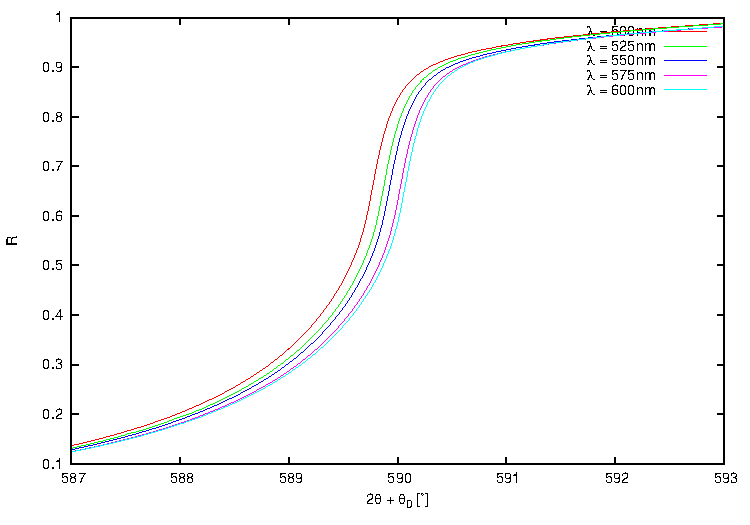
\includegraphics[width=1\textwidth]{totalreflexionen.pdf}
	\caption{Gemessene Reflektivit�ten $R$ in Abh�ngigkeit der zu kalibrierenden
	  	   		Winkelangabe des Rotationstisches $2\theta+\theta_0$ bei verschiedenen
				Wellenl�ngen $\lambda$ einfallenden Lichts.}
	\label{fig:totref}
\end{figure}

\clearpage

Wie man in Abbildung \ref{fig:totref} sehen kann, verschiebt sich die Kurve bei h�heren Wellenl�ngen in Richtung gr��eren Winkeln, was mit 
der Frequenzabh�ngigkeit der Permittivit�t von Glas $\eps_{Glas}(\lambda)$ zusammenh�ngt.

\begin{figure}[h]
    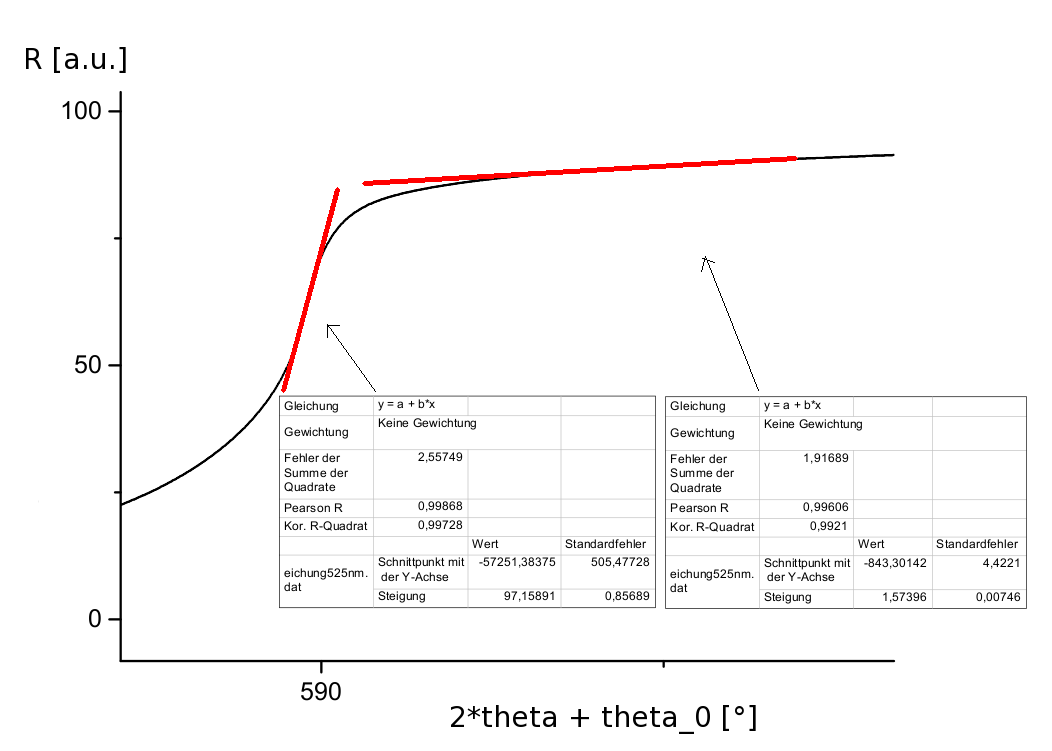
\includegraphics[width=1\textwidth]{linreg-totref-525nm.png}
	\caption{Gemessene Reflektivit�t $R$ in Abh�ngigkeit der zu kalibrierenden Winkelangabe
				des Rotationstisches $2\theta+\theta_0$ bei Wellenl�nge
				$\lambda=525\text{nm}$. In Rot die linearen Regressionen
				zur Bestimmung des Totalreflexionswinkels.}
	\label{fig:linreg}
\end{figure}

In Abbildung \ref{fig:linreg} sieht man ein Beispiel f�r den Fit, den wir an allen f�nf Kurven durchgef�hrt haben. In Tabelle \ref{tab:totref} sieht man nun
die eingestellten Wellenl�ngen, den theoretischen $\theta_{tot}$ und experimentellen Wert $\alpha_{tot}$  f�r die Totalreflexion, 
sowie den errechneten Offset $\theta_{0}$.
\newpage

\begin{table}\label{tab:totref}
\begin{tabular}[t]{|l|l|l|l|}

\hline
$\lambda$ [nm]& $\theta_{tot}$ [�] & $\alpha_{tot}$ [�] &$\theta_{0}$ [�] \cellcolor{dunkelgrau} \\
\hline
500 & 43,14 &590,05 &503,77\cellcolor{dunkelgrau}\\
\hline
525 & 43,19 &590,10 &503,72\cellcolor{dunkelgrau}\\
\hline
550 & 43,23 &590,19 &503,73\cellcolor{dunkelgrau}\\
\hline
575 & 43,27 &590,30 &503,76\cellcolor{dunkelgrau}\\
\hline
600 & 43,30 &590,19 &503,73\cellcolor{dunkelgrau}\\


\end{tabular}
\end{table}



Unser Offset den wir nun ber�cksichtigen werden lautet : $\theta_{0}= (503,74 \pm 0,02) �$